\documentclass[9pt]{article}
\usepackage[letterpaper,margin=0.55in]{geometry}
\usepackage[T1]{fontenc}
\usepackage{newtxtext,newtxmath}
\usepackage{microtype}
\usepackage{graphicx}
\usepackage{booktabs}
\usepackage{amsmath}
\usepackage{xcolor}
\usepackage{multicol}
\usepackage{enumitem}
\usepackage{titlesec}
\usepackage{caption}
\usepackage{tikz}
\usetikzlibrary{arrows.meta,positioning}
\usepackage{pgfplots}
\pgfplotsset{compat=1.18}
\usepackage[hidelinks]{hyperref}

\definecolor{ink}{HTML}{17324D}
\definecolor{rulegray}{HTML}{A8B4BC}
\setlength{\columnsep}{0.22in}
\setlength{\parindent}{0pt}
\setlength{\parskip}{1.5pt}
\setlength{\emergencystretch}{1.5em}
\pagestyle{empty}
\titleformat{\section}{\bfseries\color{ink}\fontsize{9.2}{10.2}\selectfont}{}{0pt}{}[\vspace{1.2pt}\color{rulegray}\titlerule]
\titlespacing*{\section}{0pt}{4pt}{2.5pt}
\captionsetup{font=footnotesize,labelfont=bf,skip=2pt}
\setlist[itemize]{leftmargin=1.2em,itemsep=0pt,topsep=1pt,parsep=0pt}

\newcommand{\pct}[1]{#1\%}

\begin{document}

\begin{center}
{\fontsize{16}{17}\selectfont\bfseries\color{ink} Structured Extraction from Pittsburgh 311 Waste Records}\par
\vspace{2pt}
{\fontsize{10}{11}\selectfont Comparing Local Phi, Hosted Luna, and TypeSafe JEV}\par
\vspace{5pt}
{\bfseries Rizaldy Utomo} $\cdot$ Carnegie Mellon University $\cdot$
\href{mailto:rutomo@andrew.cmu.edu}{rutomo@andrew.cmu.edu}
\end{center}

\vspace{-2pt}
\noindent\colorbox{gray!9}{\parbox{0.965\textwidth}{\small
\textbf{Abstract.} I constructed a 180-record corpus from Pittsburgh waste-service guidance, historical 311 codebooks, and operational summaries, then evaluated structured extraction on 25 seeded records. A local Phi baseline reached \pct{36} exact agreement across three fields. A targeted prompt raised service-focus agreement from \pct{72} to \pct{88}, but exact agreement rose only to \pct{40} because other errors offset part of the gain. GPT-5.6 Luna reached \pct{88} and TypeSafe JEV reached \pct{72} exact agreement on the same sample. The experiment supports human-reviewed document extraction, while the available records cannot establish resident-intake accuracy or faster physical resolution.}}

\vspace{4pt}
\begin{center}
\resizebox{0.985\textwidth}{!}{%
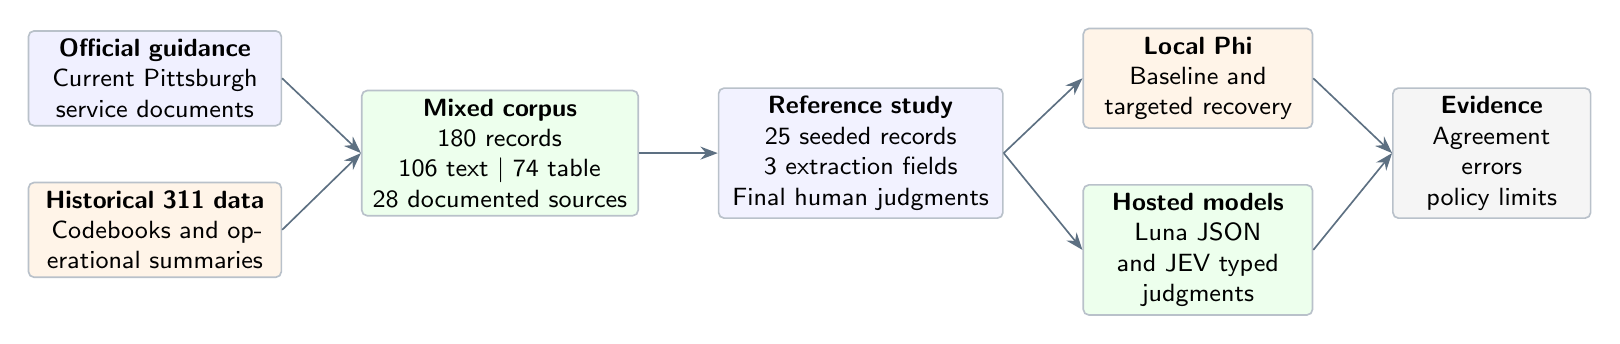
\begin{tikzpicture}[
  node distance=7mm and 10mm,
  flow/.style={-{Stealth[length=2.2mm]}, semithick, draw=ink!70},
  card/.style={rounded corners=2pt, draw=ink!30, semithick, align=center,
    minimum height=12mm, text width=30mm, inner sep=3pt, font=\sffamily\small},
  source/.style={card, fill=blue!6},
  history/.style={card, fill=orange!9},
  corpus/.style={card, fill=green!7, text width=33mm},
  study/.style={card, fill=blue!5, text width=34mm},
  model/.style={card, text width=27mm},
  evidence/.style={card, fill=black!4, text width=23mm}
]
\node[source] (guidance) {\textbf{Official guidance}\\Current Pittsburgh service documents};
\node[history, below=of guidance] (history) {\textbf{Historical 311 data}\\Codebooks and operational summaries};
\node[corpus, right=of guidance, yshift=-9.5mm] (corpus) {\textbf{Mixed corpus}\\180 records\\106 text $\mid$ 74 table\\28 documented sources};
\node[study, right=of corpus] (study) {\textbf{Reference study}\\25 seeded records\\3 extraction fields\\Final human judgments};
\node[model, fill=orange!9, right=of study, yshift=9.5mm] (phi) {\textbf{Local Phi}\\Baseline and targeted recovery};
\node[model, fill=green!7, below=of phi] (luna) {\textbf{Hosted models}\\Luna JSON and JEV typed judgments};
\node[evidence, right=of phi, yshift=-9.5mm] (evidence) {\textbf{Evidence}\\Agreement\\errors\\policy limits};
\draw[flow] (guidance.east) -- (corpus.west);
\draw[flow] (history.east) -- (corpus.west);
\draw[flow] (corpus.east) -- (study.west);
\draw[flow] (study.east) -- (phi.west);
\draw[flow] (study.east) -- (luna.west);
\draw[flow] (phi.east) -- (evidence.west);
\draw[flow] (luna.east) -- (evidence.west);
\end{tikzpicture}%
}
\captionof{figure}{Evidence path from official sources to a controlled extraction comparison. The corpus represents service documents and administrative summaries rather than original resident complaint narratives.}
\end{center}

\vspace{-3pt}
\begin{multicols}{2}
\section{Background and Question}
Pittsburgh uses 311 records to manage service requests, monitor work, and allocate resources \cite{wprdcguide}. These records are valuable administrative evidence, but reported requests reflect articulated demand and should not be read as a complete measure of neighborhood need \cite{whitetrump}. I focused on waste and neighborhood cleanliness because the domain combines current service instructions with legacy issue categories, missing definitions, and changing department labels.

I asked: \emph{How accurately can a compact local model extract service focus, information type, and explicitly named departments from this mixed corpus, and what changes after targeted prompt recovery and comparison with a lightweight hosted model?}

\section{Corpus and Task}
The corpus contains 180 distinct records from 28 documented sources: 106 natural-language sections and 74 table records. Current City guidance covers collection, missed pickup, dumping, recycling, hazardous waste, and related services. Historical WPRDC material contributes codebook rows and issue-level summaries. Every record preserves source, retrieval time, modality, and licensing context. Public access alone was not treated as an open license.

For record $i$, the extraction target was
\[
 f_{\theta}(x_i) \rightarrow
 (\hat y_i^{\mathrm{focus}},\hat y_i^{\mathrm{type}},
 \hat y_i^{\mathrm{dept}}).
\]
I made the final human judgments for a seeded sample of $n=25$ before examining Phi predictions. Codex assisted with coding and workflow suggestions. Department names were valid only when explicitly present in a record; outside knowledge was excluded.

\section{Evaluation Design}
Phi-4-mini-instruct was run locally with deterministic generation. Phi-4-mini is a compact 3.8-billion-parameter model \cite{phi4mini}. A schema validator counted malformed output as failure. Exact agreement required all three fields to match:
\[
 A_{\mathrm{exact}}=\frac{1}{n}\sum_{i=1}^{n}
 \mathbb{1}[\hat{\mathbf y}_i=\mathbf y_i].
\]
Field agreement applied the same indicator separately to each field. TF-IDF features over text and serialized tables, followed by six-cluster K-means, provided a descriptive corpus reading \cite{sklearn}. Cluster comparisons were interpreted cautiously because evaluation counts ranged from one to eight records.
\end{multicols}

\newpage
\small
\begin{center}
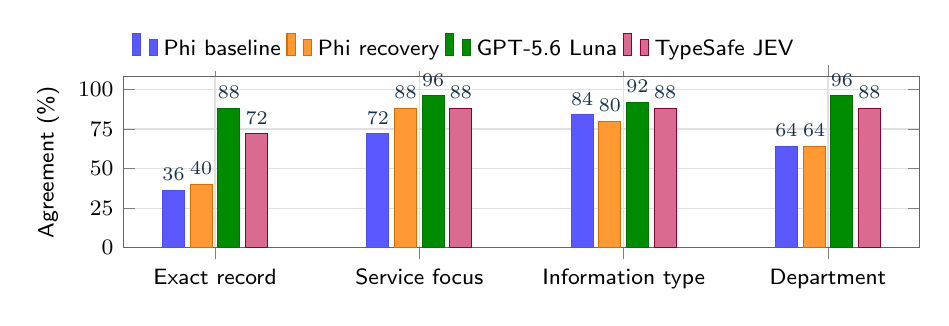
\begin{tikzpicture}
\begin{axis}[
  width=0.965\textwidth,
  height=3.75cm,
  ybar,
  bar width=8pt,
  ymin=0,
  ymax=108,
  ytick={0,25,50,75,100},
  ylabel={Agreement (\%)},
  symbolic x coords={Exact record,Service focus,Information type,Department},
  xtick=data,
  x tick label style={font=\sffamily\footnotesize},
  y tick label style={font=\sffamily\footnotesize},
  label style={font=\sffamily\footnotesize},
  legend style={at={(0,1.03)},anchor=south west,draw=none,font=\sffamily\footnotesize,legend columns=4},
  nodes near coords,
  nodes near coords style={font=\sffamily\scriptsize, color=ink},
  grid=major,
  major grid style={draw=black!12},
  axis line style={draw=black!60},
  enlarge x limits=0.15,
]
\addplot[fill=blue!65, draw=blue!70] coordinates {(Exact record,36) (Service focus,72) (Information type,84) (Department,64)};
\addplot[fill=orange!80, draw=orange!85!black] coordinates {(Exact record,40) (Service focus,88) (Information type,80) (Department,64)};
\addplot[fill=green!55!black, draw=green!45!black] coordinates {(Exact record,88) (Service focus,96) (Information type,92) (Department,96)};
\addplot[fill=purple!58, draw=purple!75!black] coordinates {(Exact record,72) (Service focus,88) (Information type,88) (Department,88)};
\legend{Phi baseline,Phi recovery,GPT-5.6 Luna,TypeSafe JEV}
\end{axis}
\end{tikzpicture}
\captionof{figure}{Agreement on the same 25 reference records. Recovery improved the targeted service-focus field by 16 percentage points, while full-record agreement increased by 4 points.}
\end{center}

\vspace{-4pt}
\noindent\begin{minipage}[t]{0.485\textwidth}
\vspace{0pt}
\section{Findings}
The Phi baseline produced valid structured output for all records but reached \pct{36} exact agreement. Field agreement was \pct{72} for service focus, \pct{84} for information type, and \pct{64} for responsible department. Valid JSON therefore did not imply correct interpretation. Phi sometimes treated a statistical source or mentioned organization as the responsible department, and it over-selected \texttt{dumping} for vague violations, commercial dumpsters, junk vehicles, and property-compliance records.

The recovery prompt required explicit evidence before assigning \texttt{dumping}. Service-focus agreement increased to \pct{88}; two records became fully correct and one previously correct record regressed. Information-type agreement declined to \pct{80}, department agreement remained \pct{64}, and exact agreement reached \pct{40}. The recovery was developed and evaluated on the same 25 records, so the four-point gain is diagnostic rather than independent generalization evidence.

GPT-5.6 Luna reached \pct{88} exact agreement using the baseline prompt and schema. Its field agreement was \pct{96}, \pct{92}, and \pct{96}, respectively. Three records still contained disagreements. The 52-point exact-agreement gap from the Phi baseline suggests model capability mattered substantially in this task, but one small same-sample run is not a general model benchmark. TypeSafe JEV 1.13.0 reached \pct{72} exact agreement and \pct{88} on each field. It used typed Choice and Noul judgments plus deterministic department candidates with complete candidate coverage \cite{typesafe}. Because this differs from Luna’s generative JSON interface, I treat it as a complementary structured-decision experiment. At September 21 prices, the 25-record JEV run cost about \$0.00079 from API-reported input tokens, versus a reconstructed Luna estimate of \$0.00282; observed mean latency was 0.19 versus 1.15 seconds.

\section{Corpus Structure}
K-means separated the corpus into seasonal recycling guidance (45 records), historical request summaries (33), graffiti and legacy codes (16), missed-pickup procedures (32), hazardous-waste and zero-waste guidance (29), and refuse codebook categories (25). Representatives were coherent enough to support these human-readable names. Baseline exact agreement ranged from zero to approximately \pct{67}, but cluster evaluation counts were too small to rank themes reliably.

\vspace{2pt}
\begin{center}
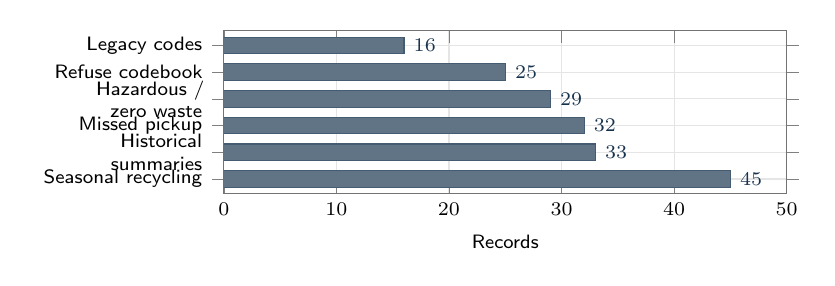
\begin{tikzpicture}
\begin{axis}[
  xbar,
  width=0.72\linewidth,
  height=3.65cm,
  xmin=0,
  xmax=50,
  xtick={0,10,20,30,40,50},
  xlabel={Records},
  symbolic y coords={Legacy codes,Refuse codebook,Hazardous / zero waste,Missed pickup,Historical summaries,Seasonal recycling},
  ytick=data,
  y dir=reverse,
  x tick label style={font=\sffamily\scriptsize},
  y tick label style={font=\sffamily\scriptsize,text width=21mm,align=right},
  label style={font=\sffamily\scriptsize},
  nodes near coords,
  nodes near coords style={font=\sffamily\scriptsize,color=ink},
  bar width=6pt,
  enlarge y limits=0.11,
  grid=major,
  major grid style={draw=black!10},
  axis line style={draw=black!55},
]
\addplot[fill=ink!68,draw=ink!80] coordinates {
  (16,Legacy codes)
  (25,Refuse codebook)
  (29,Hazardous / zero waste)
  (32,Missed pickup)
  (33,Historical summaries)
  (45,Seasonal recycling)
};
\end{axis}
\end{tikzpicture}
\captionof{figure}{Cluster sizes across all 180 corpus records. Labels were assigned after reading representative records; the clusters describe corpus structure rather than service demand.}
\end{center}

\end{minipage}\hfill
\begin{minipage}[t]{0.485\textwidth}
\vspace{0pt}
\section{Policy Interpretation}
The workflow can support document indexing, taxonomy audits, and human-reviewed metadata extraction. It should flag ambiguous records for staff instead of silently inferring current routing from older labels. The strongest operational signal is disagreement itself: a field that repeatedly fails can reveal unclear instructions, taxonomy drift, or insufficient context.

The evidence does not support autonomous 311 routing. Original resident narratives are absent, geographic reporting can be uneven, and historical categories may not represent current practice. Administrative closure duration records a status transition; it does not prove that a physical issue was resolved. A deployment study would need fresh resident-level examples, representative neighborhood coverage, a held-out evaluation set, and review of errors that could delay or misroute service.

\section{Conclusion}
Corpus design shaped the result as much as model choice. Targeted prompting corrected a recurring local error but produced only a modest exact-record gain. Luna performed best on the same sample, while JEV showed that a typed decision interface can also outperform local Phi. For municipal use, structured extraction is most defensible as inspectable decision support with human judgment and explicit evidence limits.

\begin{thebibliography}{9}\footnotesize
\setlength{\itemsep}{1pt}
\bibitem{wprdcguide} Western Pennsylvania Regional Data Center, ``City of Pittsburgh 311 Data User Guide,'' accessed Sep. 2026. \url{https://wiki.wprdc.org/wiki/City_of_Pittsburgh_311_Data_User_Guide}
\bibitem{whitetrump} A. White and K.-S. Trump, ``The Promises and Pitfalls of 311 Data,'' \emph{Urban Affairs Review}, vol. 54, no. 4, pp. 794--823, 2018. doi:10.1177/1078087416673202.
\bibitem{phi4mini} M. Abdin et al., ``Phi-4-Mini Technical Report,'' arXiv:2503.01743, 2025.
\bibitem{typesafe} TypeSafe AI, ``System One and Python SDK Documentation, accessed Sep. 2026. \url{https://docs.typesafe.ai/}
\bibitem{sklearn} F. Pedregosa et al., ``Scikit-learn: Machine Learning in Python,'' \emph{J. Mach. Learn. Res.}, vol. 12, pp. 2825--2830, 2011.
\bibitem{wprdcdata} City of Pittsburgh, ``311 Data Archive,'' WPRDC, accessed Sep. 2026. \url{https://data.wprdc.org/dataset/311-data}
\end{thebibliography}
\end{minipage}

\end{document}
